\documentclass{beamer}
\usepackage{subfig}
\usepackage{hyperref}
\hypersetup{
    colorlinks=false,
    linkcolor=blue,
    filecolor=magenta,      
    urlcolor=cyan,
}

\urlstyle{same}

\mode<presentation> {
    \usetheme{Frankfurt}
    \usecolortheme{dolphin}
    \setbeamertemplate{footline}[page number]
}

\title{\huge Vim \\
    \large Making text editing fun and efficient
}

\author{Alec Gibson}
\institute[BlueCat]
{
    BlueCat Networks \\
    \medskip
    \textit{agibson@bluecatnetworks.com}
}
\date{November 24, 2020}

\begin{document}

\begin{frame}
    \titlepage % Print the title page as the first slide
\end{frame}

\begin{frame}
    \frametitle{Disclaimer}
    \small The target audience of this talk is not seasoned users of Vi-family editors (though you are more than welcome to stay if this describes you). Many of the features I will refer to as Vim features were Vi features first. I never used Vi, and clarifying when features were introduced in Vim's lineage is outside the scope of this talk. So for the purpose of this talk \textbf{they are Vim features}.\\
    \vspace{0.5cm}
    Furthermore, everything I say in this talk applies equally to Neovim as it does to Vim. Neovim is a fork of Vim with some refactoring of the source code, slightly saner default options, no Benevolent Dictator For Life, support for lua plugins, and which tends to implement new features more quickly. I personally use Neovim instead of Vim, but both operate extremely similarly.
\end{frame}

\begin{frame}
    \frametitle{About This Presentation}
    \begin{itemize}
	\item This presentation was created in Neovim 0.5.0 using the Beamer Latex package
	\item The source code is available at \url{https://github.com/alec-gibson/vim-fun-and-efficient}
	\item For discussions about Vim, please post in the company \#vim-geeks slack channel!
    \end{itemize}
\end{frame}

\begin{frame}
    \frametitle{Overview}
    \tableofcontents
\end{frame}

\section{About Vim}
\begin{frame}
    \frametitle{About Vim}
    \tableofcontents[currentsection]
\end{frame}
\begin{frame}
    \frametitle{What is Vim}
    \centerline{\large According to vim.org}
    \vspace{0.5cm}
    \small Vim is a highly configurable text editor built to make creating and changing any kind of text very efficient. It is included as "vi" with most UNIX systems and with Apple OS X.\\
    \vspace{0.5cm}
    Vim is rock stable and is continuously being developed to become even better. Among its features are:\\
    \begin{itemize}
	\item persistent, multi-level undo tree
	\item extensive plugin system
	\item support for hundreds of programming languages and file formats
	\item powerful search and replace
	\item integrates with many tools
    \end{itemize}
\end{frame}

\begin{frame}
    \centerline{\large Here are some important features I think were missed:}
    \vspace{0.5cm}
    \small
    \begin{itemize}
	\item Vim is very lightweight, meaning it runs smoothly on any modern computer, and even performs well over SSH.
	\item Vim's startup time feels instantaneous.
	\item Because Vim runs in a terminal it works nicely with other terminal utilities (like tmux), and you can pipe the output of scripts directly into Vim.
	\item Vim's configuration is scriptable, so you can define custom functions then use them in commands and keybindings.
	\item Vim has been popular for over two decades, and its keybindings are supported in most other editors either natively or through plugins (including VSCode, Emacs, and IntelliJ to name a few)
    \end{itemize}
\end{frame}

\begin{frame}
    \centerline{\large And most importantly....}
    \vspace{0.5cm}
    \small \textbf{If you are not already using them, Vim's keybindings can teach you a new, more efficient way to edit text.}\\
    \vspace{0.5cm}
    \textit{More on these keybindings later.}
\end{frame}

\begin{frame}
    \frametitle{Who Should Try Vim?}
    \centerline{\large You may appreciate Vim if you:}
    \vspace{0.5cm}
    \begin{itemize}
	\item Spend a large amount of your day editing plain text files (common in software development and IT)
	\item Make frequent use of your terminal emulator
	\item Appreciate the value of keyboard shortcuts for everything
	\item Like to customize your tools to suit your workflow
	\item Want a more efficient way to edit text - particularly to perform boring, repetitive edits
    \end{itemize}
\end{frame}

\section{Vim 101}
\begin{frame}
    \frametitle{Vim 101}
    \tableofcontents[currentsection]
\end{frame}
\begin{frame}
    \frametitle{Entering and Exiting Vim}
\end{frame}
\begin{frame}
    \frametitle{Insert Mode}
\end{frame}
\begin{frame}
    \frametitle{Normal Mode}
\end{frame}
\begin{frame}
    \frametitle{Command-Line Mode}
\end{frame}
\begin{frame}
    \frametitle{Visual Mode}
\end{frame}
\begin{frame}
    \frametitle{How to Help Yourself}
\end{frame}

\section{Power Tools}
\begin{frame}
    \frametitle{Power Tools}
    \tableofcontents[currentsection]
\end{frame}
\begin{frame}
    \frametitle{The Jump List}
\end{frame}
\begin{frame}
    \frametitle{Text Objects}
\end{frame}
\begin{frame}
    \frametitle{Registers and Macros}
\end{frame}
\begin{frame}
    \frametitle{Substitute and Global}
\end{frame}
\begin{frame}
    \frametitle{The Undo Tree}
\end{frame}
\begin{frame}
    \frametitle{Vimscript}
\end{frame}
\begin{frame}
    \frametitle{Execute and Normal}
\end{frame}

\section{File Navigation}
\begin{frame}
    \frametitle{File Navigation}
    \tableofcontents[currentsection]
\end{frame}
\begin{frame}
    \frametitle{Buffers, Windows and Tabs}
\end{frame}
\begin{frame}
    \frametitle{Argument, Location and Quickfix Lists}
\end{frame}
\begin{frame}
    \frametitle{Grep and Vimgrep}
\end{frame}
\begin{frame}
    \frametitle{Cdo, Ldo, Argdo}
\end{frame}
\begin{frame}
    \frametitle{Finding Files Quickly}
    NOTE: discuss fuzzy finder and file tree plugins here
\end{frame}

\section{Configuration}
\begin{frame}
    \frametitle{Configuration}
    \tableofcontents[currentsection]
\end{frame}
\begin{frame}
    \frametitle{Setting Options}
\end{frame}
\begin{frame}
    \frametitle{Keybindings and Abbreviations}
\end{frame}
\begin{frame}
    \frametitle{Functions and Custom Commands}
\end{frame}
\begin{frame}
    \frametitle{Automatic Commands}
\end{frame}
\begin{frame}
    \frametitle{Plugins}
\end{frame}

\section{Links for Further Learning}
\begin{frame}
\end{frame}

\section{Goodbye}
\begin{frame}
    \centerline{\huge All Praise VI VI VI}
    \vspace{0.5cm}
    \centerline{\huge Editor of The Beast}
    \begin{figure}
	\centering
	\subfloat{{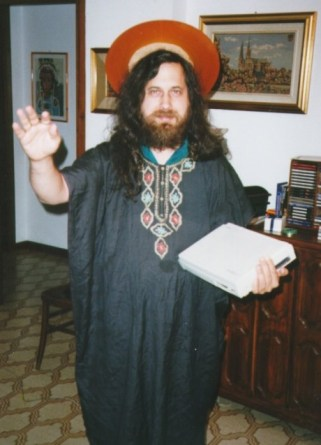
\includegraphics[width=0.3\linewidth]{saintignucius.jpg} }}% Created by Wouter van Oortmerssen
	\qquad
	\subfloat{{
\includegraphics[width=0.3\linewidth]{freebsd-daemon.png} }}% Created by Poul-Henning Kamp under the beer-ware license (https://svnweb.freebsd.org/base/head/share/examples/BSD_daemon/README?view=markup)
    \end{figure}
\end{frame}

\end{document} 
